\documentclass[12pt]{amsart}
\usepackage{amssymb,amsmath,latexsym}
\usepackage[centering,text={15.5cm,22cm},
                marginparwidth=20mm]{geometry}
\usepackage{tikz}

\usepackage[draft, layout=margin]{fixme}
\fxsetup{theme=color}
\FXRegisterAuthor{ss}{ass}{SS}
\FXRegisterAuthor{mc}{amc}{MC}
\FXRegisterAuthor{mg}{amg}{MG}
\newcommand\mandy[1]{{\color{blue} \sf $\clubsuit\clubsuit\clubsuit$ Mandy: [#1]}}
\newcommand\markg[1]{{\color{red} \sf $\clubsuit\clubsuit\clubsuit$ Mark: [#1]}}

\newtheorem{lemma}{Lemma}[section]
\newtheorem{theorem}{Theorem}[section]
\newtheorem{propo}[theorem]{Proposition}
\newtheorem{prop}[theorem]{Proposition}
\newtheorem{cor}[theorem]{Corollary}
\newtheorem{conj}[theorem]{Conjecture}
\newtheorem{claim}[theorem]{Claim}
\newtheorem{claim*}{Claim}
\newtheorem{rmk}[theorem]{Remark}
\newtheorem{thm}[theorem]{Theorem}
\newtheorem{defn}[theorem]{Definition}

\theoremstyle{remark}
\newtheorem{example}[theorem]{Example}
\newtheorem{remark}[theorem]{Remark}
\newtheorem{question}[theorem]{Question}

\newcommand{\QQ}{\mathbb{Q}}
\newcommand{\ZZ}{\mathbb{Z}}
\newcommand{\NN}{\mathbb{N}}
\newcommand{\RR}{\mathbb{R}}
\newcommand{\cA}{\mathcal{A}}
\newcommand{\Hom}{\operatorname{Hom}}
%%%%%%%%%%%% mathfrak
\newcommand{\dd}{\mathfrak{d}}
\newcommand{\fod}{\mathfrak{d}}
\newcommand{\DD}{\mathfrak{D}}
\newcommand{\fom}{\mathfrak{m}}
\newcommand{\gr}{\mathrm{gr}}
\newcommand{\Mono}{\operatorname{Mono}}
%%%%%%%%%%%%%%%%%%%%%%%%%%%%%%%%%%%%%%%%%%%%%%%%%%%%%%%%%%%%%%%%%%%
\title{Theta functions and greedy bases}
\author{CCGMMRSW}

\begin{document}
\maketitle

\section{Scattering diagrams and broken lines}
In this section, we will describe the cluster algebras $\cA (b,c)$ from 
the point of view of scattering diagrams. While all the results in this section
are derived from \cite{GHKK}, we will adopt a slightly simplified notation
from that used in \cite{GHKK} as it is sufficient for the rank $2$ case.

Let $N = \ZZ^2$ be a lattice, $M = \Hom (N, \ZZ)$. Write $M_{\RR} = M \otimes 
\RR$, $N_{\RR} = N\otimes \RR$. Take $\Bbbk$ to be a 
field of characteristic 0. Fix a basis $f_1, f_2$ of $M$, and let
$\sigma \subseteq M_{\RR}$ be a strictly convex rational polyhedral
cone. We let $P=\sigma \cap M$, and write $\widehat{\Bbbk[P]}$ for the
completion of the monoid ring $\Bbbk[P]$ at the maximal monomial ideal
$\fom$
generated by $\{z^m \,|\, m\in P\setminus\{0\}\}$.
Given $m\in M$, we can write $z^m \in \Bbbk[M]$ as
$A_1^{a_1} A_2^{a_2}$ if $m=a_1f_1+a_2f_2$.

\begin{defn}
\label{walldef}
A \emph{wall} is a pair $(\dd, f_{\dd})$, where 
\begin{itemize}
    \item $\dd \subseteq M_{\mathbb{R}}$ is either a ray $\RR_{\le 0}m_0$ 
or a line $\RR m_0$ with $m_0\in \sigma \cap(M\setminus 0)$;
    \item $f_{\dd} \in \widehat{\Bbbk [P]}$ such that
    \[ f_{\dd} = 1 + \sum_{k\geq 1} c_k z^{k m_0},\]
    for some $c_k \in \Bbbk$. 
\end{itemize}
The set $\dd \subseteq M_{\mathbb{R}}$ is called the support of the wall $(\dd, f_{\dd})$.
\end{defn}

\begin{defn}
A scattering diagram $\DD$ is a collection of walls such that for each $k \geq 0$, the set
\[  \{ (\dd, f_{\dd})\, |\, f_{\dd} \neq 1 \bmod \fom^k   \}\]
is finite. 
\end{defn}

For a scattering diagram $\DD$, we denote the support of $\DD$ as
\[\text{Supp} (\DD) := \bigcup_{\dd \in \DD} \dd. \]

Consider a smooth immersion
\[  \gamma: [0,1] \rightarrow M_{\mathbb{R}} \backslash  \{0 \}  \]
with endpoint not in the support of $\DD$. Assume $\gamma$ is transversal to each wall of $\DD$ that it crosses. For each power $k \geq 1$, we can find the
longest sequence of numbers
$ 0< t_1 \leq t_2 \leq \cdots \leq t_s < 1 $ with $\gamma(t_i)\in\dd_i$
for some $i$ with
$f_{\dd_i} \neq 1 \text{ mod } \fom^k   $ and $\dd_i\not=\dd_j$ whenever
$t_i=t_j$. For each $i$, define $\theta_{\dd_i}\in {\mathrm{Aut}}_{\Bbbk-alg}\big(
\widehat{\Bbbk[P]}\big)$ as
\[\theta_{\dd_i} (z^m) = z^m f_{\dd_i}^{\langle m, n_0 \rangle }, \]
where $n_0 \in N$ is primitive, annihilates the tangent space to $\dd_i$, and is uniquely determined by the sign convention $ \langle n_0, \gamma'(t_i) \rangle <0$. 
Take $\theta^k_{\gamma, \DD} := \theta_{\dd_s} \circ  \cdots \circ \theta_{\dd_1}$.We can then define the \textit{path-ordered product} as
\[\theta_{\gamma, \DD} = \lim_{k \rightarrow \infty} \theta ^k_{\gamma, \DD}. \]

\begin{defn}
A scattering diagram is \emph{consistent} if $\theta _{\gamma, \DD}$ only depends on the endpoints of $\gamma$ for any path $\gamma$ for which $\theta _{\gamma, \DD}$ is well defined.
\end{defn}

\begin{theorem}(Kontsevich-Soibelman) \label{KS}
Given a scattering diagram $\DD$, there always exists a consistent scattering diagram $\DD'$ which contains $\DD$ such that $\DD'\setminus\DD$ only consists of
rays.
\end{theorem}


%%%%%%%%%%%%%%%%%%%% Scattering diagram
We now explain the scattering diagram associated to each cluster algebra 
$\cA (b,c)$ using the techniques of \cite{GHKK}. 
This cluster algebra is determined by the skew-symmetrizable exchange matrix
$\epsilon = \begin{pmatrix} 0 & c\\ -b & 0\end{pmatrix}$,
where $b$, $c$ are positive integers. 

Following Example 1.30 of \cite{GHKK}, we take
$\sigma$ to be the second quadrant, i.e., the cone generated by $-f_1$ and
$f_2$. Then the scattering diagram associated
to the above exchange matrix is
\[\DD_{\mathrm{in},(b,c)} := \big\{\big( \RR(1,0), 1+A_1^{-b}\big), \big(\RR(0,1), 
1+A_2^c\big) \big\}.\]

From Theorem~\ref{KS}, we can obtain a consistent scattering diagram $\DD_{(b,c)}$ 
associated to $\DD_{\mathrm{in},(b,c)}$.

\begin{example} \label{ex}
Consider $\epsilon =  \begin{pmatrix}
0 &1 \\
-1 &0
\end{pmatrix}$. 
Then we get
\[\DD_{\mathrm{in},(1,1)} =  \{ (\RR e_1, 1+A_1^{-1}), (\RR e_2, 1+A_2)  \}   \]
and the associated scattering diagram (shown in Figure~\ref{fig:diagex}) is
\[ \DD_{(1,1)} = \DD_{\mathrm{in},(1,1)} \cup \{\RR_{\geq 0} (1,-1), 1+A_1^{-1}A_2  \}.   \]

\begin{figure}
\centering
\begin{tikzpicture}
\draw
(-2,0) -- (2,0) node[right] {$1+A_1^{-1}$}
(0,-2) -- (0,2) node[left] {$1+A_2$}
(0,0) -- (2,-2) node[below] {$1+A_1^{-1}A_2$};
\end{tikzpicture}
\caption{The scattering diagram for Example~\ref{ex}} \label{fig:diagex}
\end{figure}
\end{example}

For general $b$ and $c$, the diagram $\DD_{(b,c)} \backslash 
\DD_{\mathrm{in},(b,c)}$ may 
consist of an infinite number of rays, and in fact is infinite precisely
when $bc\ge 4$. A more detailed description of the rays which appear
can be found in \cite{GHKK}, Example 1.30. We summarize the crucial
points here.
The first observation is that all rays in $\DD_{(b,c)} \backslash 
\DD_{\mathrm{in},(b,c)}$
are contained in the fourth quadrant and are not contained in one of the
coordinate axes. Now consider two linear operator
$S_1 =  
\begin{pmatrix}
-1 & -b \\
0& 1
\end{pmatrix}
$
and
$S_2 =  
\begin{pmatrix}
1 & 0 \\
-c & -1
\end{pmatrix}
$.
Then if $(\dd, f_{\dd}(z^m)) \in \DD_{(b,c)} \backslash \DD_{\mathrm{in},(b,c)}$
and $S_i (\dd)$ is contained strictly in the fourth quadrant, then 
$(S_i(\dd), f_{\dd}(z^{S_i(m)})) \in \DD_{(b,c)} \backslash 
\DD_{\mathrm{in},(b,c)}$. 
So $\DD_{(b,c)} \backslash \DD_{\mathrm{in},(b,c)}$ is invariant under $S_1$, $S_2$. 
Applying $S_2$ to $\{ (\RR_{\geq 0}(1,0), 1+A_1^{-b}) \}$ or $S_1$ to 
$(\RR_{\geq 0}(0,-1), 1+A_2^c)  \}$ gives us rays in $\DD_{(b,c)} \backslash 
\DD_{\mathrm{in},(b,c)}$. Continuing to iterate the compositions of $S_1$ and $S_2$, 
the rays will converge to the rays with slopes $-\frac{bc \pm \sqrt{bc(bc-4)}}{2b}$. This gives a complete description of the rays outside of the cone spanned by the two rays. Inside the cone, it is likely that there is a non-trivial
ray of every possible rational slope. 
\mcnote{more detail at end?}\mgnote{Wait and see what other facts we need about
the diagram.} The chamber structure one sees outside of the quadratic 
irrational cone is very well-behaved and familiar in the theory of
cluster algebra. This chamber structure coincides with the Fock-Goncharov 
cluster complex, see \cite{GHKK}, \S2, the mutation fan of Reading \cite{R}, 
and the picture group of Igusa-Orr-Todorov-Weyman \cite{IOTW}.

\begin{figure}
\input{diagram33.pstex_t}
\caption{The general appearance of the scattering diagram in case $bc>4$.}
\label{diagram33}
\end{figure}

The following result explains the connection betwen scattering diagrams
and the corresponding cluster algebra:

\begin{theorem}
\label{univLaurent}
Let $\DD:=\DD_{(b,c)}$ as constructed above.
Let $f \in \Bbbk[M]$ be a Laurent polynomial. For any path
$\gamma$ for which $\theta_{\gamma,\DD}$ is defined, $\theta_{\gamma,\DD}(f)$
can be viewed as an element of $\Bbbk[[A_1,A_2^{-1}]]$ localized at 
$A_1A_2^{-1}$. Then $f$ is a universal Laurent polynomial for the initial
seed data if, for any path $\gamma$ in $M_{\RR}$ with starting
point in the first quadrant and endpoint in one of the chambers of
$\DD$, $\theta_{\gamma,\DD}(f)$ in fact lies $\Bbbk[M]$.
\end{theorem}

\begin{proof}
This is a special case of \cite{GHKK}, Theorem 4.4.
\end{proof}

We will now define broken lines. Broken lines were introduced in 
\cite{G10} as a way of describing holomorphic disks which appear in
mirror symmetry in a tropical manner. Their theory was further developed
in \cite{CPS}, and then used in \cite{GHK11} and \cite{GHKK} to construct
canonical bases in various circumstances.

\begin{defn} \label{brokendef}
Let $\DD$ be a scattering diagram, $m_0 \in M \backslash \{0\}$ and $Q \in M_{\RR} \backslash \text{Supp}(\DD)$. A broken line for $m_0$ with endpoint $Q$ is a
continuous, proper, and  piecewise linear path $\gamma : ( - \infty , 0] 
\rightarrow M_{\mathbb{R}} \backslash \{ 0\} $ with a finite number of domains 
of linearity, along with a choice of
monomial $c_L z^{m_L} \in \Bbbk[M]$ attached to each domain of linearity $L \subseteq ( - \infty, 0]$ of $\gamma$. The path $\gamma$ and the monomial $c_L z^{m_L}$ need to satisfy the following conditions:
\begin{itemize}
    \item $\gamma(0) = Q$.
    \item If $L$ is the first (i.e., unbounded) domain of linearity of $\gamma$, then $c_L z^{m_L} = z^{m_0}$.
    \item For $t$ in a domain of linearity, $\gamma'(t) = -m_L$.
    \item $\gamma$ bends only when it crosses a wall. If $\gamma$ bends between the domain of linearity $L$ to $ L'$ when crossing $(\dd, f_{\dd})$, then $c_{L'}z^{m_{L'}}$ is a term in $\theta_{\gamma, \dd} (c_L z^{m_L})  $.
\end{itemize}
\end{defn}

\begin{defn}
Let $\DD, m_0, Q$ as in Definition~\ref{brokendef}. For a broken line $\gamma$ with initial slope $m_0$ and endpoint $Q$, denote $I(\gamma) = m_0$ and $b(\gamma) = Q$. Define
\[\Mono (\gamma) = c(\gamma)z^{F(\gamma)}\]
to be the monomial $c_L z^{m_L}$ attached to the last domain of linearity $L$ of $\gamma$. We further define
\[ \vartheta_{Q, m_0} = \sum_{\gamma} \Mono (\gamma), \]
where the sum is over all broken lines for $m_0$ with endpoint $Q$.
\end{defn}


\begin{example} \label{brokenex}
Consider the scattering diagram with $b=c=2$. Let us consider broken lines for initial slope $m_0 = (1,-1)$ with endpoint $Q= (1.5,1)$. First of all, we can have a broken line $\gamma_1$ which does not bend. This is shown as red in Figure~\ref{figbrokenex}. Then
\[\Mono(\gamma_1) = A_1 A_2^{-1}.\]
There is the other broken line $\gamma_2$ which bends at the $x$-axis as shown 
as blue ray in Figure~\ref{figbrokenex}. Since
\[ \theta_{\gamma_2, \RR(1,0)} (A_1 A_2^{-1}) = A_1 A_2^{-1}(1+A_1^{-2}) =  A_1 A_2^{-1} + A_1^{-1} A_2^{-1} . \]
So to bend, we choose the second term and obtain a broken line
$\gamma_2$ with $\Mono(\gamma_2) =  A_1^{-1} A_2^{-1}$. The last borken
line $\gamma_3$ bends at the $x$ and $y$-axes, the latter
bend coming from
\[ \theta_{ \gamma_3, \RR(0,1)} ( A_1^{-1} A_2^{-1}) =  A_1^{-1} A_2^{-1} + A_1^{-1} A_2.  \]
This time we have $\Mono (\gamma_3) = A_1^{-1} A_2$. Thus given $m_0 = (1,-1)$ with endpoint point $Q= (1.5,1)$, 
\[ \vartheta_{Q,(1,-1)} =  A_1 A_2^{-1} + A_1^{-1} A_2^{-1} +A_1^{-1} A_2 .  \]


\begin{figure}
\centering
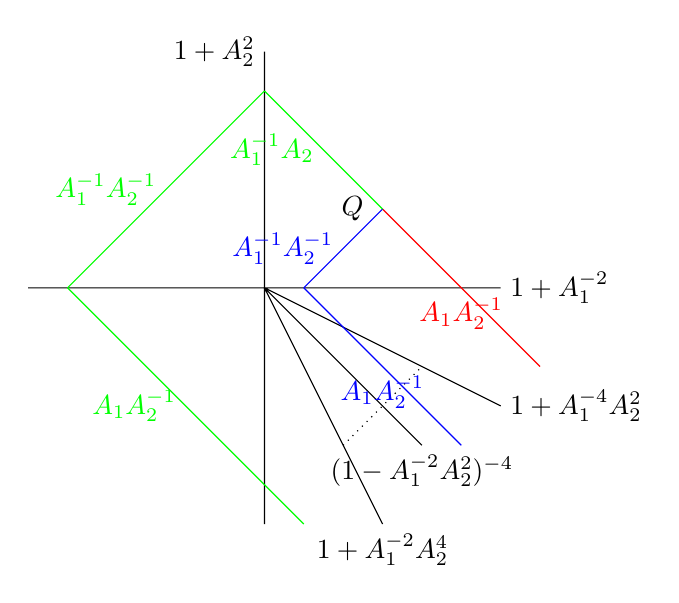
\begin{tikzpicture}
\draw
(-3,0) -- (3,0) node[right] {$1+A_1^{-2}$}
(0,-3) -- (0,3) node[left] {$1+A_2^2$}
(0,0) -- (3,-1.5) node[right] {$1+A_1^{-4}A_2^2$}
(0,0) -- (2,-2) node[below] {$(1-A_1^{-2}A_2^2)^{-4}$}
(0,0) -- (1.5,-3) node[below] {$1+A_1^{-2}A_2^4$};

\draw
(1.5,1) node[circle, left] {$Q$};

\draw[dotted]
(1,-2) -- (2,-1);


\draw[red]
(3.5,-1) --node[below]{$A_1 A_2^{-1}$} (1.5,1);

\draw[blue]
(0.5,0) -- node[left] {$A_1^{-1} A_2^{-1}$}  (1.5,1)
(0.5,0) -- node[below] {$A_1 A_2^{-1}$} (2.5,-2);

\draw[green]
(0,2.5)  -- node[left] {$A_1^{-1}A_2$} (1.5,1)
(-2.5,0) -- node[left] {$A_1^{-1} A_2^{-1}$}  (0,2.5)
(0.5, -3)  --node[left] {$A_1 A_2^{-1}$} (-2.5,0);

\end{tikzpicture}
\caption{Example~\ref{brokenex}} \label{figbrokenex}
\end{figure}

\end{example}




The following summarizes the relevant main points of the theta functions defined
above as shown in \cite{GHKK}:

\begin{theorem} 
\begin{enumerate}
\item
If $\DD$ is any consistent scattering diagram,
$Q$, $Q'$ are two general points on $M_{\RR} \backslash$ Supp$(\DD)$, and 
$\gamma$ is a path joining $Q$ and $Q'$, then 
\[\theta_{\gamma, \DD }(\vartheta_{Q,m_0}) = \vartheta_{Q', m_0}. \]
\item Taking $\DD=\DD_{(b,c)}$, 
if $Q$ lies in the interior of a chamber of $\DD$, then 
$\vartheta_{Q,m_0}$ is a Laurent polynomial.
\item Taking $\DD=\DD_{(b,c)}$, for $Q$ in the interior of the first
quadrant, $\vartheta_{Q,m_0}$ is
a universal Laurent polynomial.
\item Taking $\DD=\DD_{(b,c)}$, if $m_0$ lies in the interior of a chamber of 
$\DD$, and $Q$ lies in the same chamber, then $\vartheta_{Q,m_0}=z^{m_0}$.
\end{enumerate}
\end{theorem}

\begin{proof}
(1) is a main result of \cite{CPS}, and quoted in this context in
\cite{GHKK}, Theorem 3.5. The second statement follows from
\cite{GHKK}, Proposition 8.26. Next, (3) follows from (2) by Theorem
\ref{univLaurent}. Finally, (4) follows from \cite{GHKK}, Proposition 3.8
(and see the argument of \cite{GHKK}, Theorem 4.8 in the case that
the chamber is not the positive quadrant.)
\end{proof}

\begin{remark}
If $m_0\in M$ lies in one of the chambers of $\DD_{(b,c)}$, and $Q$ lies
in the first quadrant, then from (1) and (4) of the above theorem, 
$\vartheta_{Q,m_0}=\theta_{\gamma,\DD_{(b,c)}}(z^{m_0})$ for a path 
$\gamma$ joining a chamber containing $m_0$ to $Q$. In fact it follows
from the details of the proof of Theorem \ref{univLaurent} 
that $\vartheta_{Q,m_0}$
is in fact a cluster monomial. It follows from \cite{GHKK}, Theorem 7.5,
that the ${\bf g}$-vector of this cluster monomial is precisely $m_0$.
\end{remark}

\begin{example} 
Let us try one more calculation of broken line. We take the same scattering diagram as in example~\ref{brokenex}. Now take the initial slope $m_0$ as $(2,-2)$ with the same endpoint $Q= (1.5,1)$. By similar calculation, 
\[ \vartheta _{Q, (2,-2)}= A_1^2 A_2^{-2} + A_1^{-2}A_2^2 + A_1^{-2}A_2^{-2} + 2 A_2^{-2} + 2A_1^{-2}.  \]
Note that 
\[ \vartheta _{Q, (2,-2)} = (\vartheta_{Q,(1,-1)}) ^2 -2. \]
In this $b=c=2$ scattering diagram $\DD$, the ray with slope $(1,-1)$ does not lie in any chamber in $\DD$. So neither $\vartheta_{Q,(1,-1)}$ nor 
$\vartheta _{Q, (2,-2)}$ are cluster monomials.

There are a number of known bases for $\cA(2,2)$, which give different results
for the basis elements with ${\bf g}$-vector $(d,-d)$ for $d>0$. This
calculation shows that at least for $d=1$ or $2$, theta functions agree
with the greedy basis.
\end{example}


\section{Relation to greedy bases}

For studying the relation of theta functions to greedy bases,
instead of using the scattering diagram $\DD_{(b,c)}$ described in the
previous section, we will use a closely related scattering diagram 
$\DD_{\mathrm{gr},(b,c)}$.
To relate $\DD_{(b,c)}$ with $\DD_{\gr,(b,c)}$, let $e_1,e_2$ be the
dual basis of $f_1, f_2$, and define a mapping 
$T:M \rightarrow M$ given by
\[
T (m) := 
\begin{cases}
    m   & \langle e_2 , m \rangle \geq 0 \\
    m + b f_1 \langle e_2, m \rangle & \langle e_2, m \rangle \leq 0.
\end{cases}
\]
Denote
\[ \mathcal{H}_{+} = \{  m \in M_{\mathbb{R}}\, |\, \langle e_2 , m \rangle \geq 0  \}, \qquad \mathcal{H}_{-} = \{  m \in M_{\mathbb{R}} \,|\, \langle e_2 , m \rangle \leq 0  \}.\]
We denote by $T_+$ or $T_-$ the linear extension of $T|_{\mathcal{H}_+}$
or $T|_{\mathcal{H}_-}$ respectively.
We further define $T_{\pm}$ to act on a power 
series in $\widehat{\Bbbk[P]}$ by applying $T_{\pm}$ to each exponent of the 
power series. 

We define $\DD_{\gr,(b,c)} := T(\DD_{(b,c)})$ by 
\begin{itemize}
    \item replacing each wall $(\fod,f_{\fod})\in \DD_{(b,c)}\setminus
\DD_{\mathrm{in},(b,c)}$ with $(T_-(\fod), T_-(f_{\fod}))$;
    \item replacing the wall $(\RR f_1, 1+z^{(-b,0)})$ with 
$(\RR f_1, 1+z^{(b,0)})$;
    \item replacing the wall $(\RR f_2, 1+z^{(0,c)})$ with two walls,
$(T_+(\RR_{\ge 0} f_2), T_+(1+z^{(0,c)}))$ and $(T_-(\RR_{\le 0}f_2),
T_-(1+z^{(0,c)}))$.
\end{itemize}

\begin{remark}
A priori the wall $(T_+(\RR_{\ge 0}f_2),T_+(1+z^{(0,c)}))$ does not
fit the definition of wall in Definition~\ref{walldef}. However, 
by Example \ref{ex}, the ray of $\DD_{(b,c)}\setminus
\DD_{\mathrm{in},(b,c)}$ with the largest slope is the ray
$(\RR_{\ge 0} (b,-1),1+A_1^{-cb}A_2^c)$, with slope $-1/b$. This ray 
is taken to  $(\RR_{\ge 0}(0,-1),1+A_2^c)$ by $T$. 
Thus we see that in fact all other rays in the 
fourth quadrant are moved to the third quadrant by $T$. 
Furthermore, the two
rays $(\RR_{\ge 0} (0,1), 1+A_2^c)$ and $(\RR_{\ge 0}(0,-1), 1+A_2^c)$
can then be replaced by a single line $(\RR (0,1), 1+A_2^c)$. 
From this it follows that
$\DD_{\gr,(b,c)}$ is a scattering diagram for the cone $\sigma_{\gr}$
generated by $f_1, f_2$, i.e., the first quadrant. 
Then $\DD_{\gr,(b,c)}\supseteq\DD_{\gr,\mathrm{in},(b,c)}$ where
\[
\DD_{\gr,\mathrm{in},(b,c)}=\big\{\big(\RR(1,0), 1+A_1^b\big), 
\big(\RR (0,1), 1+A_2^c\big)\big\}
\]
and 
$\DD_{\gr,(b,c)}\setminus\DD_{\gr,\mathrm{in},(b,c)}$ consists only of rays
in the third quadrant. One can show using a suitable uniqueness statement
for the construction of Theorem \ref{KS} that $\DD_{\gr,(b,c)}$
is produced from $\DD_{\gr,\mathrm{in},(b,c)}$ using that theorem.
\end{remark}

\begin{theorem}
$T$ defines a one-to-one correspondence between broken line for $m_0$ with endpoint $Q$ for $\DD_{(b,c)}$ and broken lines for $T(m_0)$ with endpoint $T(Q)$ for $\DD_{\gr,(b,c)}$. For $Q \in \mathcal{H}_{k,+}$ or $\mathcal{H}_{k,-}$, we have
\[ 
\hbox{$\vartheta^{\gr}_{T(Q),T( m_0)} = T_{+} (\vartheta_{Q, m_0})$
or $T_{-} (\vartheta_{Q, m_0})$}\]
respectively.
\end{theorem}

\begin{proof}
This is essentially the same as the argument of \cite{GHKK}, Prop.\ 3.6.
Given a broken line $\gamma$ for $\DD:=\DD_{(b,c)}$, we denote its image as 
under $T$ as $T(\gamma)$: this is the broken line whose underlying map
is $\gamma\circ T$. Furthermore, we can assume all the domains of linearity 
$L$ of $\gamma$ satisfy either $\gamma(L) \subseteq \mathcal{H}_{+} $ or $
\gamma(L)\subseteq \mathcal{H}_{-}$ by subdividing $L$. We then change
the monomial attached to the domain of linearity $L$ by applying either
$T_+$ or $T_-$ to the exponent in the two cases.
To prove the statement, we only need to check the bending at $\RR f_1$. Let $L_1$, $L_2$ be the domains of linearity of $\gamma$ before and after bending along
$\RR f_1$. So $c_{L_2} z^{m_{L_2}}$ is a term in
$\theta (c_{L_1} z^{m_{L_1}}) = c_{L_1} z^{m_{L_1}} (1+z^{-bf_1}) ^{|\langle  e_2, m_{L_1}  \rangle|} $. 

First, assume $\gamma$ passes from $\mathcal{H}_-$ to $\mathcal{H}_+$. In this case, we would have $\langle e_2 , m_{L_1} \rangle < 0$, or else $L_1$ would
not intersect $\RR f_1$. Now in order for the monomial $c_{L_2}z^{T_+(m_{L_2})}
=c_{L_2}z^{m_{L_2}}$
attached to $L_2$
in $T\circ\gamma$ to satisfy the bending rule, it must be a term in
\begin{align*} 
c_{L_1} z^{T_-(m_{L_1})} (1+z^{bf_1}) ^{-\langle  e_2, T_-(m_{L_1}) \rangle} & =
c_{L_1} z^{m_{L_1}+bf_1\langle e_2, m_{L_1}\rangle} (1+z^{bf_1}) ^{-\langle  e_2, 
m_{L_1}+bf_1\langle e_2, m_{L_1} \rangle \rangle} \\
& = c_{L_1} z^{m_{L_1}} (1+z^{-bf_1}) ^{-\langle  e_2, m_{L_1}  \rangle}.
\end{align*}
This shows that $T_k(\gamma)$ satisfies the correct rule when bending along
$(\RR f_1, 1+z^{(b,0)})$. By repeating similar calculation, we can see that this also holds when $\gamma$ passes from $\mathcal{H}_+$ to $\mathcal{H}_-$.
\end{proof}

The following demonstrates the utility of using $\DD_{\gr,(b,c)}$:

\begin{prop}
If $m_0\in M$ and $Q$ lies in the first quadrant, then 
\[
\vartheta^{\gr}_{Q, m_0}=z^{m_0}(1+f(A_1,A_2))
\]
where $f\in (A_1,A_2)\subseteq \Bbbk[A_1,A_2]$.
In particular, $m_0$ is the ${\bf d}$-vector of $\vartheta^{\gr}_{Q,m_0}$.
\end{prop}

\begin{proof}
There is always a broken line whose image is $\RR_{\ge 0}m_0+Q$, with
the single attached monomial $z^{m_0}$. Thus $z^{m_0}$ appears as a term
in $\vartheta^{\gr}_{Q,m_0}$. However, because the functions attached
to any ray or line of $\DD_{\gr,(b,c)}$ are of the shape $1+g(A_1,A_2)$
with $g(A_1,A_2) \in (A_1,A_2) \subseteq \Bbbk[[A_1,A_2]]$, it follows
that any term coming from a broken line which bends must be of the form
$cz^{m_0}A_1^{d_1}A_2^{d_2}$ with $d_1,d_2\ge 0$, $d_1+d_2>0$. This proves
the result.
\end{proof}

\mgnote[layout=inline]{It might be appropriate to add stuff about the quantum version here.
Right now I don't know if we can easily prove enough facts about the
quantum version for our main result. I suggest we wait until the rest
is written up and then I see whether it is possible to extend the proof
given what we currently know. (For example, in general I don't know how
to get the chamber structure that is visible in the classical case.)}



\begin{thebibliography}{99}
\bibitem[CPS]{CPS} M.~Carl, M.~Pumperla, and B.~Siebert,
A tropical view of Landau-Ginzburg models, available at
http://www.math.uni-hamburg.de/home/siebert/preprints/LGtrop.pdf
\bibitem[G10]{G10} M.~Gross,  \emph{Mirror symmetry for $\mathbb{P}^2$ 
and tropical geometry}, Adv.\ Math., {\bf 224} (2010), 169--245.
\bibitem[GHK11]{GHK11} M.~Gross, P.~Hacking and S.~Keel, \emph{Mirror
symmetry for log Calabi-Yau surfaces I}, preprint, 2011.
\bibitem[GHKK]{GHKK} M.~Gross, P.~Hacking, S.~Keel, M.~Kontsevich,
\emph{Canonical bases for cluster algebras}, preprint, 2014.
\bibitem[IOTW]{IOTW} K.~Igusa, K.~Orr, G.~Todorov, J.~Weyman \emph{Picture groups of finite type and cohomology in type $A_n$}, preprint, available at 
http://people.brandeis.edu/~igusa/Papers/PictureGroup.pdf
\bibitem[R]{R} N.~Reading, \emph{Universal geometric cluster algebras}, Mathematische Zeitschrift, {\bf 277 } (2014), 499-547.
\end{thebibliography}

\end{document}

%sagemathcloud={"zoom_width":125}

